\section{Studio di fattibilità}

\subsection{Contesto d'uso}
Dalle analisi precedenti di user research e valutazione di sistemi
esitenti si può fare un quadro del contesto d'uso dell'applicazione
proposta.
Vedremo in particolare qual'è il target d'utenza, quali sono i task da
prendere in considerazione e quali sono i possibili vincoli tecnici e
ambientali.

\subsubsection{Target d'utenza}
Come emerge dalla user research il target d'utenza previsto è molto
eterogeneo, infatti non si sono riscrontrati dei ristrettivi limiti di
età, istruzione o competenze culinarie.\\
Forse l'unica vera restrizione riguarda la nazionalità degli utenti
in quanto si è deciso di concentrare
l'attenzione verso l'utenza italiana. Questa scelta è nata dall'analisi
delle statistiche le quali suggeriscono che l'Italia è una delle
prime nazioni nel mondo per quanto riguarda la passione culinaria
\ref{fig:cooking-country}. A conoscenza di ciò, focalizzarsi su un
utenza internazionale avrebbe potuto confondere gli italiani, poco familiari
con lo stile culinario non tradizionale. Ad esempio la colazione
italiana prevede un pasto molto rapido a differenza di molte colazioni
estere e la suddivisione delle portate in ``primo'' e ``secondo'', le quali
identificano già la categoria della pietanza, non è molto comune
all'estero.

\subsubsection{Task}
A seguito delle valutazioni dei sistemi esistenti, è risultato opportuno
rivisitare la lista dei task già definita nello user research
\ref{tasks}, con
l'idea di far forza sul contesto nel quale le applicazioni esistenti
mostrano le loro debolezze.
TODO modificare lista task:

\begin{enumerate}
\label{newtasks}
\item Ricerca di una ricetta per nome.
\item Ricerca di una ricetta per ingredienti.
\item Filtro di una ricetta per categoria.
\item Filtro di una ricetta in base alle intolleranze/allergie.
\item Suggerimenti sulle ricette di stagione.
\item Salvare una ricetta nei preferiti.
\item Rimuovere una ricetta dai preferiti.
\item Distinguere le varie fasi di una preparazione della ricetta.
\item Visualizzare le foto inerenti alla preparazione di
una ricetta.
\item Avanzare con le fasi di preparazione mediante messaggi vocali.
\item Text-to-Speech delle fasi di preparazione di una ricetta.
\item Individuare gli ingredienti necessari alla preparazione di una
ricetta.
\item Individuare la difficoltà di preparazione di una ricetta.
\item Inserire una nuova ricetta nel catalogo dell'applicazione.
\item Condividere una ricetta sui social network.
\item Commentare una ricetta in un apposito topic online.
\item Accedere alla lista della spesa.
\item Inserire gli ingredienti nella lista della spesa.
\item Rimuovere gli ingredienti dalla lista della spesa.
\item Modificare la grandezza del font di una ricetta.
\item Creare un menù completo selezionando una lista di ricette.
\item Selezionare la lingua dell'applicazione.
\end{enumerate}

\subsubsection{Vincoli tecnici ed ambientali}
L'applicazione è pensata per essere utilizzata in ambienti probabilmente
molto caotici, in cui l'attenzione dell'utente potrebbe essere
facilmente catturata da altri elementi del contesto. Questo aspetto è
stato riscontrato anche durante le osservazioni del contextual inquiry:
i tre studenti si sono facilmente distratti a causa dell'euforia della
novità, mentre la signora Antonietta si è fatta distrarre dalla
discussione con la sorella. A rafforzare tale supposizione sono i
risultati del sondaggio i quali mostrano che il livello di esperienza
culinaria media è medio-bassa.
Un vincolo per l'appliczione
potrebbe essere infatti la disposizione disordinata degli ingredienti
e degli atrezzi nella cucina, che potrebbe impediere un comodo
raggiungimento e utilizzo del
device, scoraggiando l'utente all'approccio tecnologico. Inoltre
avere le mani impegnate potrebbere rendere l'applicazione inutilizzabile
in alcuni casi, soprattuto se l'ausilio dei comandi vocali non fosse
previsto. Ad ogni modo anche nche nel caso in cui fossero previsto comandi vocali,
un ambiente molto caotico potrebbe essere un vincolo.\\
Il tutto suggerisce di progettare un applicazione la cui interfaccia sia
molto semplice, immediata e che riduca il carico di stress
percepito dall'utente.
\subsection{Personas}

\begin{table}[H]
	\begin{centering}
	\begin{tabular} { | r  p{10cm} | }
		\hline
		\multirow{2}{*}{
			\begin{minipage}{.18 \textheight}
				\vspace{0.1in}
				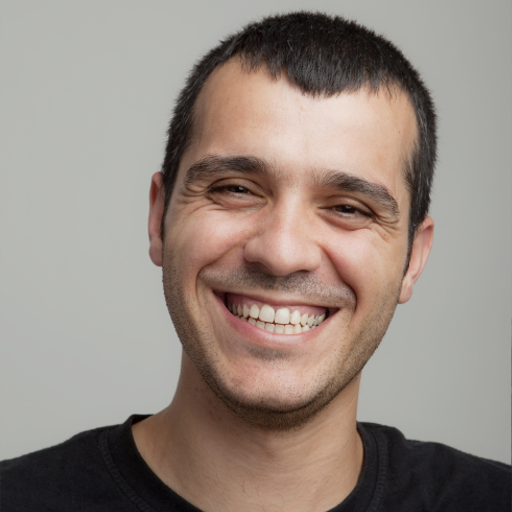
\includegraphics[width=\linewidth]{img/personas/filippo.png}
			\end{minipage}
		}
		 & \vspace{0.1 in}\Large\textbf{Filippo} \\ 
		& \vspace{0.1 in}\large{\emph{``Anche se viaggio molto per catturare il mondo,
cucinare all'estero mi fa
		sentire sempre a casa. Sempre pronto a re-inventare la tradizione anche con
		ingredienti difficili.''}}\\[8ex] 
		\hline
		\textbf{Anni} & 36 \\ \hline
		\textbf{Occupazione} & Fotografo \\ \hline
		\textbf{Famiglia} & {Nonostante i frequenti viaggi, ha uno
studio e un domicilio a Rimini, città in cui è cresciuto con la sua
famiglia. Ogni circa due settimane Filippo fa visita ai genitori per il
pranzo domenicale insieme alla sua ragazza spagnola con cui convive.} \\
\hline
		\textbf{Profilo Tecnico} & Dopo il liceo artistico ha vissuto 5
anni in Spagna, lavorando sia come cameriere in un ristorante italiano
sia come impiegato in un'agenzia di viaggi. Tornato in italia ha poi
deciso di seguire la sua passione per la fotografia iscrivendosi
all'accademia delle belle arti. Terminati gli studi ha iniziato a
viaggiare in tutto il mondo pubblicando le sue foto in un blog wordpress gestito
da lui stesso. Da 2 anni ha aperto un proprio studio fotografico in
Italia. \\ \hline
		\textbf{Hobby} & Ha sempre avuto una grande passione per il
rugby, sport che ha abbandonato dopo l'università anche se continua a
seguirlo assiduamente. \\ \hline
		\textbf{Rapporto con la cucina} & Nonostante gli piaccia molto
la cucina spagnola e quella asiatica, rimane molto legato alla cucina
tradizionale italiana. Cucina spesso e volentieri piatti italiani molto
semplici ma che comunque sono molto graditi dalla sua ragazza spagnola.
\\ \hline
		\textbf{Rapporto con la tecnologia} & Prima di quest'anno non
aveva mai considerato
l'acquisto di un tablet, essendo abituato ad utilizzare sempre il laptop 
per necessità d'utilizzo dei software di editing
d'immagini. Dopo avero provato un tablet surface, che permette di
passare in modalità desktop aggangiando una tastiera al dispositivo, ha
deciso di comprarne uno, affascinato dalla possibilità di poter
continuare ad utilizzare i suoi software con interfaccia destkop e
sfruttare allo stesso tempo l'estrema mobilità e le app di un tablet.
Ha anche una buona familiarità con il Web avendo gestito in passato un proprio
blog di foto ed una pagina facebook. Lo scorso natale la ragazza le ha
regalato uno smartwatch che inizialmente non trovava di particolare
utilità, ma dopo aver visto che gli permette di visualizzare a distanza
la ripresa della fotocamera del suo smartphone ha iniziato ad
utilizzarlo regolarmente come supporto alla fotografia. Infatti ha
intenzione di acquistare prossimamente una nuova reflex con sistema
operativo Android da integrare al suo smartwatch.
\\ \hline
	\end{tabular}
	\end{centering}
\end{table}


\begin{table}[H]
	\begin{centering}
	\begin{tabular} { | r  p{10cm} | }
		\hline
		\multirow{2}{*}{
			\begin{minipage}{.18 \textheight}
				\vspace{0.1in}
				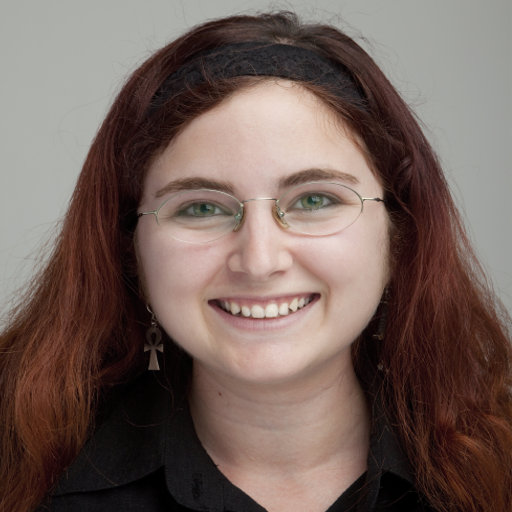
\includegraphics[width=\linewidth]{img/personas/flora.png}
			\end{minipage}
		}
		 & \vspace{0.1 in}\Large\textbf{Flora} \\ 
		& \vspace{0.1 in}\large{\emph{``I love dogs as much as I
love Italian guys. They are all handsome and funny and I am trying to
	lose some weight to look prettier. Maybe some of them will notice
me.''}}\\[8ex] 
		\hline
		\textbf{Anni} & 28 \\ \hline
		\textbf{Occupazione} & Dottoranda in geologia \\ \hline
		\textbf{Famiglia} & {Ha vissuto a Glasgow in Scozia con la madre
ed il fratello maggiore fino ai tempi del liceo. Si è poi trasferita in
un campus ad
Edimburgo per frequentare l'università. Data la breve distanza tra le
due città non ha sofferto il distacco dalla famiglia tornando a casa
quasi ogni fine-settimana. Da due anni ha lasciato la Scozia e le manca molto il
fratello con cui ha un rapporto molto speciale maturato dopo il
divorzio dei genitori.} \\
\hline
		\textbf{Profilo Tecnico} & Si è specializzata in geologia presso
l'università di Edimburgo. Ha ottenuto poi una borsa di studio per un
dottorato di ricerca all'Università di Bologna. Non ha mai lavorato al
di fuori dell'ambito accademico.\\ \hline
		\textbf{Hobby} & Ama i cani e prendersi cura di loro. Nel
fine-settimana lavora occasionalmente come dog-sitter, non molto per
bisogni economici ma per passare un po' di tempo con i cani visto che ha
dovuto lasciare il suo terrier in Scozia. \\\hline
		\textbf{Rapporto con la cucina} & Come tutti gli scozzesi ama
la cucina italiana, in particolare il gelato e la lasagna. Nei
primi mesi di dottorando in Italia ha messo su qualche chilo e ha deciso
quindi di iniziare una dieta. Spesso però, soprattuto nei periodi dalle
scadenze accademiche, non riesce a resistere ad una buona pizza o alla
trattoria bolognese,
sia per dare sfogo allo stress, sia per l'impegno di fare spesa e
cucinare.\\ \hline
		\textbf{Rapporto con la tecnologia} & Utilizza quotidianamente
il PC per fare ricerca e lo smartphone per messaggiare con gli amici.
Quando è a casa predilige il tablet perchè spesso effettua lunghe
videochiamate con la madre con cui comunica anche durante lo svolgimento
di altre mansioni, spostandosi da una stanza all'altra.\\ \hline
		\textbf{Altri particolari} & Condivide un appartamento con altri
due studenti molto più piccoli di lei. Periodicamente organizzano feste
in casa anche infrasettimanalmente. Lei ormai stanca delle feste
universitarie che si prolungano fino a tarda notte, si fa spesso ospitare
da un'amica in queste occassioni. Anche se prova una sorta di disagio per il
disturbo creato all'amica, ritiene sia l'unico modo per affrontare la giornata
succesiva.\\ \hline
	\end{tabular}
	\end{centering}
\end{table}

\begin{table}[H]
	\begin{centering}
	\begin{tabular} { | r  p{10cm} | }
		\hline
		\multirow{2}{*}{
			\begin{minipage}{.18 \textheight}
				\vspace{0.1in}
				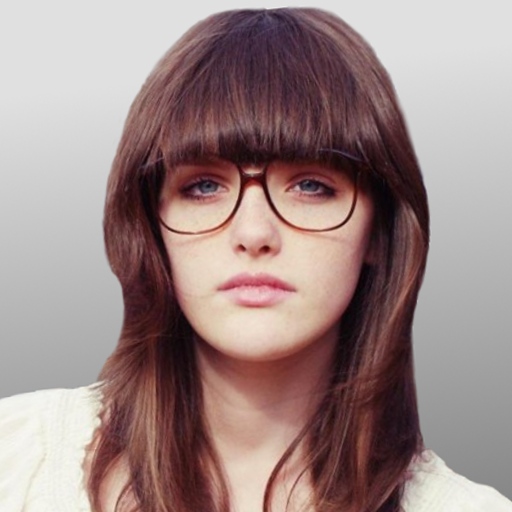
\includegraphics[width=\linewidth]{img/personas/francesca.png}
			\end{minipage}
		}
	 	& \vspace{0.1 in}\Large\textbf{Francesca} \\ 
		& \vspace{0.1 in}\large{\emph{``Ho una gran passione per l'indie rock e
il vintage design. Da due anni ho deciso di diventare vegetariana, sia
per rispettare la mia salute sia per contrastare lo sfruttamento animale
delle multinazionali.''}}\\[8ex] 
		\hline
		\textbf{Anni} & 27 \\ \hline
		\textbf{Occupazione} & Giornalista tirocinante \\ \hline
		\textbf{Famiglia} & È figlia unica ed è stata cresciuta 
a Verona dai genitori, che le hanno permesso sempre di inseguire le sue
passioni.\\ \hline
		\textbf{Profilo Tecnico} & Dopo aver terminato il liceo classico
di Verona, si è trasferita a Bologna per frequentare l'università.
Laureata da un anno in lettere e filosofia ha iniziato da qualche mese
un tirocinio retribuito in una nota testata giornalistica a Bologna. \\\hline
		\textbf{Hobby} & Nel tempo libero le piace cucire sciarpe e
capelli per lei e per il suo ragazzo. Il finesettimana non perde mai un
concerto indie rock e frequenta spesso i negozi dell'usato per alla
ricerca di oggettistica vintage. \\ \hline
		\textbf{Rapporto con la cucina} & È diventata vegeteriana dopo
aver lasciato Verona. Il suo cambio di alimentazione non è stato
drastico in quanto non le è mai piaciuta molto la carne. Il problema le
si presenta quando mangia fuori casa con altre persone, occasioni in cui
prestare attenzione agli ingredienti delle pietanze che mangia. \\ \hline
		\textbf{Rapporto con la tecnologia} & Si è sempre definita
riluttante alla tecnologia, prediligendo canali d'informazione più
classici rispetto al web. Ha utilizzato il PC per lunghi periodi
solamente per scrivere le sue tesi universitarie. Non possiede uno
smartphone e continua ancora ad utilizzare gli SMS.\\ \hline
		\textbf{Altri particolari} & Frequenta da pochi mesi un ragazzo
amante di cucina tipica emiliana. Nonostante i loro tipi di
alimentazione molto diversi, il cibo non è mai una causa di discussione. \\\hline
	\end{tabular}
	\end{centering}
\end{table}

\begin{table}[H]
	\begin{centering}
	\begin{tabular} { | r  p{10cm} | }
		\hline
		\multirow{2}{*}{
			\begin{minipage}{.18 \textheight}
				\vspace{0.1in}
				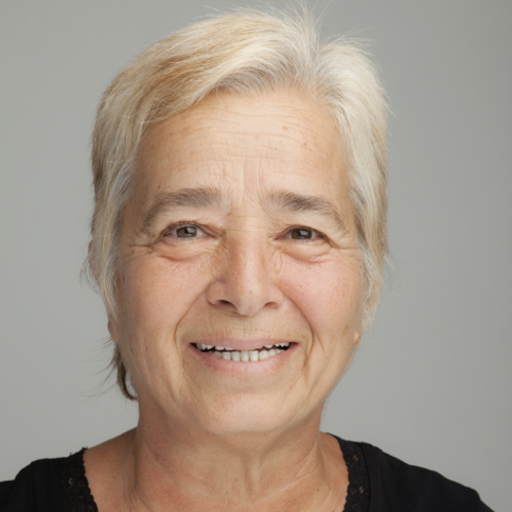
\includegraphics[width=\linewidth]{img/personas/maria.png}
			\end{minipage}
		}
	 	& \vspace{0.1 in}\Large\textbf{Maria} \\ 
		& \vspace{0.1 in}\large{\emph{``I miei figli vivono tutti in
città, ma io la montagna proprio non la lascio. Qui l'aria è buona e si
mangia bene, altro che i faste fud dove vanno i miei nipoti. Almeno con
il nuovo tablet che mi hanno regalato li vedo spesso con l'internet.''}}\\[8ex] 
		\hline
		\textbf{Anni} & 63 \\ \hline
		\textbf{Occupazione} & Pensionata \\ \hline
		\textbf{Famiglia} & Ha due figli maschi ed una femmina. I due
maschi vivono entrambi a Milano mentre la figlia vive a Napoli dopo
essersi sposata con un carabiniere conosciuto durante un suo periodo di servizio a
Milano. Quasi una volta al mese i figli di Milano vanno a trovarla a
Cusio, un piccolo paesino di montagna in provincia di Bergamo dove
tutt'ora vive. La signora Maria però, soffre molto la distanza con
l'altra figlia che riesce a vedere solo una volta l'anno durante le
feste natalizie. \\ \hline
		\textbf{Profilo Tecnico} & Ha lavorato per tutta la vita come
postina a Cusio e nei dintorni. Adesso si gode una meritata pensione. \\ \hline
		\textbf{Hobby} & Ha sempre avuto la passione per il ballo, che
coltiva con suo marito frequentando occasionalmente la balera del paese.
Oltre al liscio ha una vera ossessione per le telenovelas e tutti i
programmi TV condotti da Maria De Filippi.  \\\hline
		\textbf{Rapporto con la cucina} & A detta dei nipotini, abituati
alla cucina di città, la nonna Maria è la cuoca
più brava del mondo. Abituata ad una cucina molto tradizionale e
montana, il suo piatto forte sono i fagottini con funghi porcini e
Bitto, un formaggio di mucca tipico della Lombardia. Purtroppo il
marito della figlia che vive a Napoli è intollerante al lattosio e
quando c'è anche lui a tavola questo piatto diventa un tabù.\\ \hline
		\textbf{Rapporto con la tecnologia} & Non ha mai utilizzato un
computer. Per molto tempo i figli milanesi hanno cercato di farle
utilizzare uno
smartphone ma con scarso successo in quanto Maria, a causa
dell'abbassamento della vista, ha riscontrato che si stanca molto
	durante l'interazione con i piccoli schermi degli smartphone. I
figli hanno deciso quindi di regalarle un tablet in quanto ha uno schermo più
grande rispetto agli smartphone e molte applicazioni pensate appositamente per gli anziani.
Alla signora Maria sembra piaciere il nuovo dispositivo e, nonostante abbia dei 
tempi molto lenti di apprendimento, è molto motivata ad
imparare come utilizzarlo in quanto le permette di
videochiamare la figlia che vive a Napoli e vedere le foto dei nipotini
mentre crescono. \\ \hline
		\textbf{Altri particolari} & Il marito della signora Maria è
molto orgoglioso delle sue origini nordiche e non ha mai preso in
simpatia il carabiniere napoletano che la figlia ha sposato. \\\hline

	\end{tabular}
	\end{centering}
\end{table}

\begin{table}[H]
	\begin{centering}
	\begin{tabular} { | r  p{10cm} | }
		\hline
		\multirow{2}{*}{
			\begin{minipage}{.18 \textheight}
				\vspace{0.1in}
				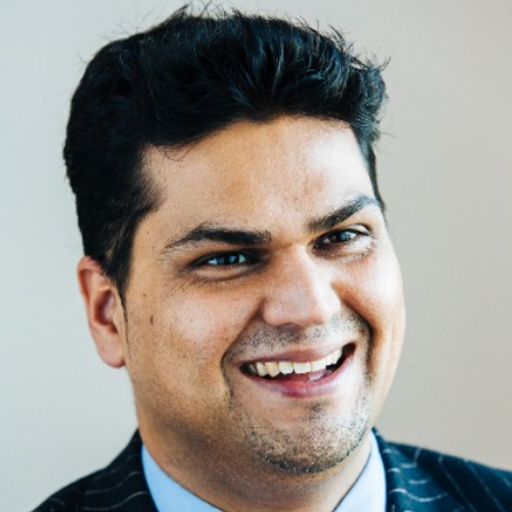
\includegraphics[width=\linewidth]{img/personas/giuseppe.png}
			\end{minipage}
		}
	 	& \vspace{0.1 in}\Large\textbf{Giuseppe} \\ 
		& \vspace{0.1 in}\large{\emph{``I milanesi parlano tutti male di
Napoli, ma dopo esserci stati non se ne vogliono più andare. Mia moglie
milanese infatti adesso ama la mia città tanto quanto ama me. Solo noi abbiamo il
sole, il mare, la pizza e il babà.''}}\\[8ex]
		\hline
		\textbf{Anni} & 42 \\ \hline
		\textbf{Occupazione} & Maresciallo dei Carabinieri \\ \hline
		\textbf{Famiglia} & Ha sposato Chiara, una donna del nord
Italia, conosciuta durante un periodo di servizio a Milano. Hanno una
bambina di 6 anni.\\ \hline
		\textbf{Profilo Tecnico} & Dopo le scuole superiori si
arruola all'Accademia Militare per intraprendere gli studi in
Giurisprudenza e diventare un ufficiale. Viene in seguito reclutato come
maresciallo dell'Arma dei Carabinieri. Attualmente è in comando stabile
presso una caserma della periferia di Napoli. \\\hline
		\textbf{Hobby} & Fuori servizio, quando non passa del tempo con
la sua famiglia, pratica il tiro con l'arco.\\ \hline
		\textbf{Rapporto con la cucina} & È di buona forchetta e gli
piace molto cucinare. Ha una buona esperienza con i fornelli maturata
durante il periodo dell'Accademia Militare e ama i piatti tipici
Napoletani e gli ingredienti del sud Italia. Negli ultimi anni però il
medico gli ha proibito di consumare latticini a causa di un intolleranza al
lattosio. Giuseppe ha impiegato diverso tempo per accettare la sua
intolleranza avendo avuto sempre un debole per la mozzarella di bufala.\\ \hline
		\textbf{Rapporto con la tecnologia} & Utilizza il PC in caserma
esclusivamente tramite il sistema software dei Carabinieri per risolvere
le pratiche quotidiane. A casa utilizza sporadicamente il
laptop della moglie giusto per navigare e riprodurre video. Possiede uno
smartphone ma lo utilizza principalmente per le classiche telefonate e fotografare i
piatti ai ristoranti.\\ \hline
	\end{tabular}
	\end{centering}
\end{table}
\subsection{Scenari d'uso}
%TODO francesca è l'amica hipster di flora da cui va a dormire. flora le
%vuole preparare una cena italiana ma francesca è vegana.

%TODO nello scenario maria litiga col marito perchè il napoletano
%giuseppe sta
%per arrivare senza preavviso e non si possono fare più i fagottini che
%tanto piacciono al suo nipote milanese preferito. Il marito di maria sostiene
%che il napoletano non è intollerante ma gli fanno male le mozzarelle
%campane perchè contaminate dai rifiuti nel sottosuolo, mentre potrebbe
%mangiare il buonissimo e incontaminato Bitto. Con l'app maria trova
%un'alternativa con un formaggio senza lattosio, dicendo al marito che
%c'è del vero Bitto dicendogli però di "mentire" al napoletano.

